\begin{figure}[ht]
  \caption[Compare the efficiency of the proposed method and the naive algorithm]{This plot shows the total runtime of the naive algorithm and the proposed method to compute the unique columns as can be seen in Table~\ref{table:efficiency_csv-70percent}. The tables were saved in a CSV format.} % TODO: better caption
  \label{fig:efficiency-base_experiment-plot} % chktex 24
  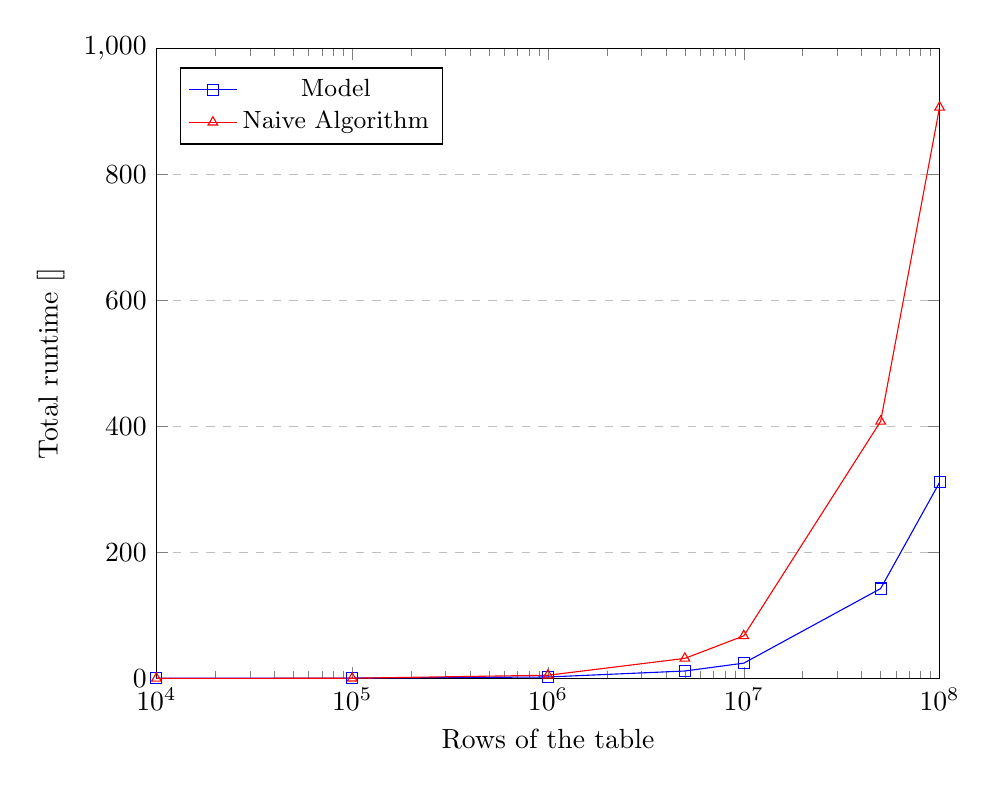
\begin{tikzpicture}
    \begin{axis}[
        % title={},
        xlabel={Rows of the table},
        ylabel={Total runtime [\si{\second}]},
        xmin=10000, xmax=100000000, xmode=log,
        ymin=0, ymax=1000,
        % xtick={0,1000,100000,10000000,100000000},
        % ytick={0,20,40,60,80,100,120},
        legend pos=north west,
        ymajorgrids=true,
        grid style=dashed,
        scale only axis,
        width={\linewidth-62pt},
        height=8cm
      ]

      \addplot[
        color=blue,
        mark=square,
      ]
      coordinates {
          (100.0,1.0835406184196472) (1000.0,0.4514627978205681) (10000.0,0.4591604061424732) (100000.0,0.5741918832063675) (1000000.0,2.2600879333913326) (5000000.0,11.771335251629353) (10000000.0,24.25790297240019) (50000000.0,142.64984269440174) (100000000.0,311.1732710637152)
        };
      \addplot[
        color=red,
        mark=triangle,
      ]
      coordinates{
          (100.0,0.0039823874831199) (1000.0,0.0037141181528568) (10000.0,0.0264939442276954) (100000.0,0.3022922314703464) (1000000.0,5.0495885498821735) (5000000.0,31.796920645982027) (10000000.0,67.54112743958831) (50000000.0,408.1332451477647) (100000000.0,906.6464131213723)
        };
      \legend{\small Model, \small Naive Algorithm}

    \end{axis}
  \end{tikzpicture}
\end{figure}
